\section{Auditorium and room acoustics}

\bi

\i This section briefly discusses issues related to the 
acoustical properties of rooms and auditoria.

\i We will pay particular attention to the distinction
between direct, reflected, and reverberant sound.
We will also learn how to calculate the reverberation
time of a room.

\i \demo Watch the YouTube video
{\tt https://www.youtube.com/watch?v=BYBSA9v8IRE}
about anechoic (i.e., echo-free) chambers.

\i \demo For a general introduction to architectural
and environmental acoustics, listen to 
``One man's quest to find the sonic wonders of the world,"
on NPR's `Fresh Air' program with Terry Gross.

\ei
%%%%%%%%%%%%%%%%%%%%%%%%%%%%%%%%%%%%%%%%%%%%%%%%%%%%%
\subsection{Direct sound}
\bi

\i {\em Direct sound} is the sound that is 
received from a source in the absence of any reflections.
See Figure~\ref{f:direct_sound}.
%
\begin{figure}[htbp]
\begin{center}
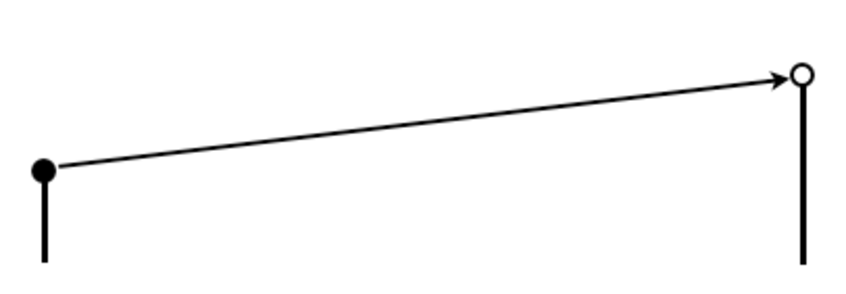
\includegraphics[width=0.6\textwidth]{reflection_0}
\caption{Direct sound only.
No reflections.}
\label{f:direct_sound}
\end{center}
\end{figure}
%

\i In an anechoic chamber (or in empty space) one 
hears only the direct sound from a source.

\i For an omni-directional source, the power is spread
out uniformly over the area of a sphere.
The intensity at a distance $r$ from a source with 
power $W$ is given by
%
\be
I = \frac{W}{4\pi r^2}
\ee
%
(Recall: intensity is the amount of energy per unit
time that passes through a unit area directed perpendicular
to the flow.)

\i \exer Calculate the power received by the ear of
a listener standing a distance of 10~m from an
omni-directional 1~watt source.
Approximate the human ear as a square with side length
of 5~cm.

\i \ans
The area of the ear is given by 
$A_{\rm ear} = (.05~{\rm m})^2 = 0.0025~{\rm m}^2$.
Since the absorbed power is equal to the intensity times
the area,
%
\be
W_{\rm ear} = I A_{\rm ear} 
=\frac{W}{4\pi r^2}\, A_{\rm ear}
=\frac{1}{4\pi 10^2} 0.0025
= 2\times 10^{-6}~{\rm watts}
\ee
%
Note that the ratio of the received power to the source
power is $2\times 10^{-6}$ or 1/500,000, which is a
very small fraction of the radiated power.

\i For a directional source, which radiates only over a 
portion of the sphere,
%
\be
I = \frac{Q W}{4\pi r^2}
\ee
%
where $Q$ is the {\em directivity factor}.
For a directional source, both $I$ and $Q$ depend on 
the direction from the source.
 
\i \ex
For a source that radiates only in a hemisphere, e.g.,
a loudspeaker mounted to the ceiling, $Q=2$.
For a source that radiates only in an octant, e.g., 
a loudspeaker in a corner, $Q=8$.

\ei
%%%%%%%%%%%%%%%%%%%%%%%%%%%%%%%%%%%%%%%%%%%%%%%%%%%%%
\subsection{Reflected sound}
\bi

\i {\em Reflected sound} is the sound that is received 
from a source after it has been reflected from one or more surfaces.

\i Recall that sound reflects according to the formula that
the angle of incidence equals the angle of reflection.
The reflected sound appears to come from an image source, as shown
in Figure~\ref{f:reflection_floor}.
%
\begin{figure}[htbp]
\begin{center}
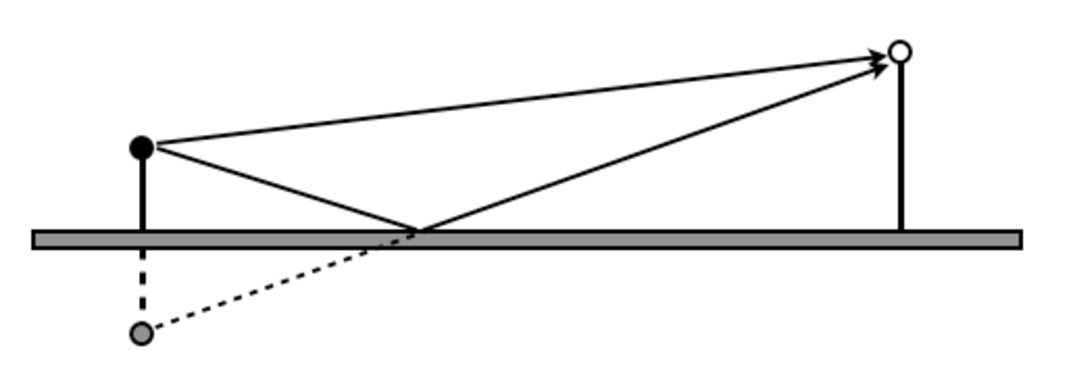
\includegraphics[width=0.7\textwidth]{reflection_floor}
\caption{Direct sound plus reflection off a floor.
The reflected sound appears to come from an image
source on the other side of the floor.}
\label{f:reflection_floor}
\end{center}
\end{figure}
%

\i {\em Specular reflection} occurs when the wavelength of sound 
is much larger than the length scale of the roughness of the surface.
Parallel rays in become parallel rays out.

\i {\em Diffuse reflection} occurs when the wavelength of sound
is of order or less than the length scale of the roughness of the surface.
Parallel rays in become non-parallel rays out.

\i Since the reflected sound travels farther than the 
direct sound, it will arrive later than the direct sound.
(The speed of sound is approximately 340~m/s in air at room temperature.
This corresponds to roughly 1000~ft/s or 1 foot per millisecond.)

\i The brain interprets the reflected sound and the direct sound 
to be the same if the time between the reception of the reflected 
and direct sound is less than $\sim\!35~{\rm msec}$.
Longer delays give rise to an echo.

\i A related phenomenon is the {\em precedence effect}:
The brain interprets the source of sound to be in the direction 
from which the first sound is heard.

\i Since the reflected sound travels farther
than the direct sound, the sound intensity level of the reflected
sound will be less than that for the direct sound.
Non-zero absorption by the reflecting wall will also reduce 
the sound intensity level.

\i \exer
A listener stands 4~m in front of a 1~watt omni-directional loudspeaker.
It is 1.5~m from a reflecting wall.

(a) Calculate the time of arrival for both the 
direct and reflected sound.

(b) Calculate the decrease in sound intensity level 
for the reflected sound relative to the direct sound,
assuming perfect reflection.

(c) Calculate the decrease in sound intensity level 
due to a non-zero absorption coefficient, e.g., $a = 0.2$.

\i \ans

(a) Using geometry, one can show that the distance that the 
reflected sound travels is $\sqrt{4^2+3^2}=5~{\rm m}$:
%
\be
t_{\rm direct}=\frac{4~{\rm m}}{346~{\rm m/s}}=12~{\rm msec}\,,
\qquad
t_{\rm reflected}=\frac{5~{\rm m}}{346~{\rm m/s}}=15~{\rm msec}
\ee

(b) The decrease in SIL comes from the increased distance 
from the source for the reflected sound:
%
\be
\Delta{\rm SIL} 
= 10\log[1/(r_{\rm reflected}/r_{\rm direct})^2]~{\rm dB}
= 10\log[(4/5)^2]~{\rm dB} 
= -2~{\rm dB}
\ee

(c) For a non-zero absorption coefficient $a=0.2$:
%
\be
\Delta{\rm SIL} 
= 10\log(1-a)~{\rm dB}
= 10\log 0.8~{\rm dB}
= -1~{\rm dB}
\ee

\ei
%%%%%%%%%%%%%%%%%%%%%%%%%%%%%%%%%%%%%%%%%%%%%%%%%%%%%%%%%%%%%%%%%
\subsection{Multiple reflections}
\bi

\i Since a room has multiple walls, a ceiling, and a floor, 
sound can undergo multiple reflections when traveling from
the source to a listener.
 
\i Figures~\ref{f:reflection_floor_ceiling},
\ref{f:reflection_floor_wall},
\ref{f:reflection_floor_wall_ceiling} show paths for 
multiple reflections.
The situation gets complicated very quickly!!
%
\begin{figure}[htbp]
\begin{center}
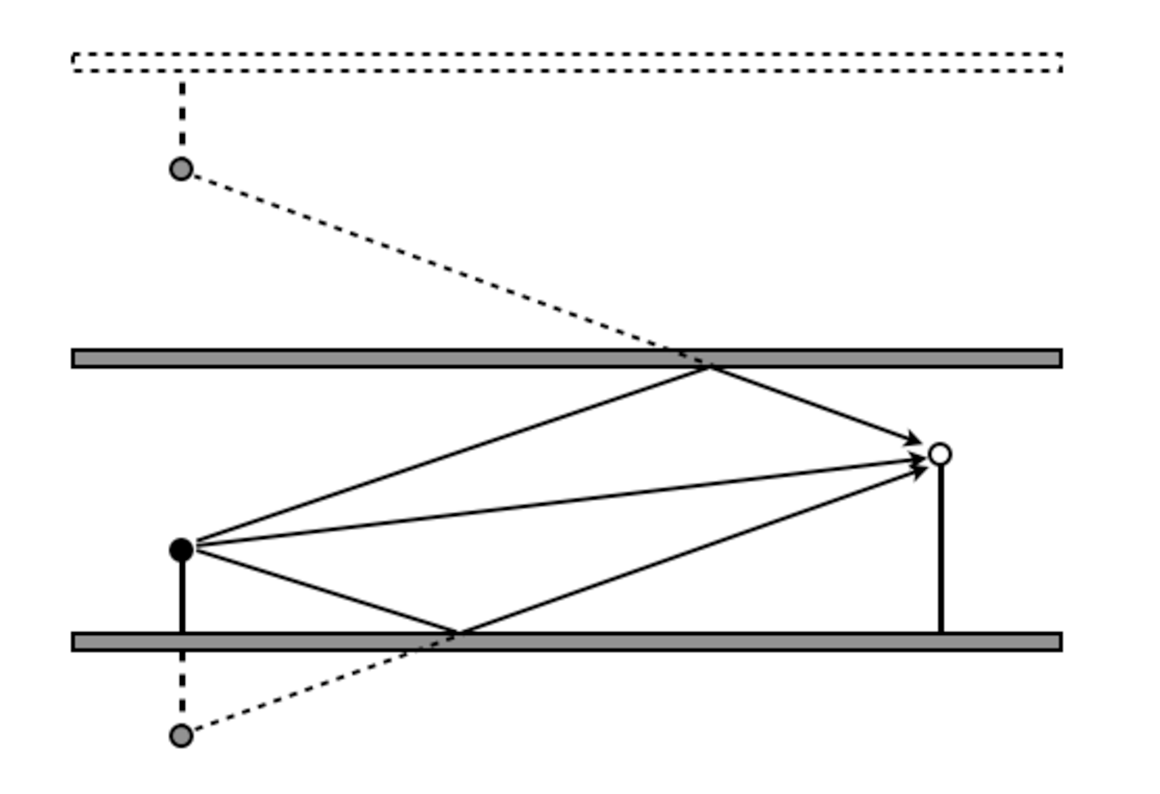
\includegraphics[width=0.7\textwidth]{reflection_floor_ceiling}
\caption{Direct sound plus reflections off a floor and a ceiling.
The reflected sound appears to come from image
sources on the other side of the floor and the other side 
of the ceiling.}
\label{f:reflection_floor_ceiling}
\end{center}
\end{figure}
%
%
\begin{figure}[htbp]
\begin{center}
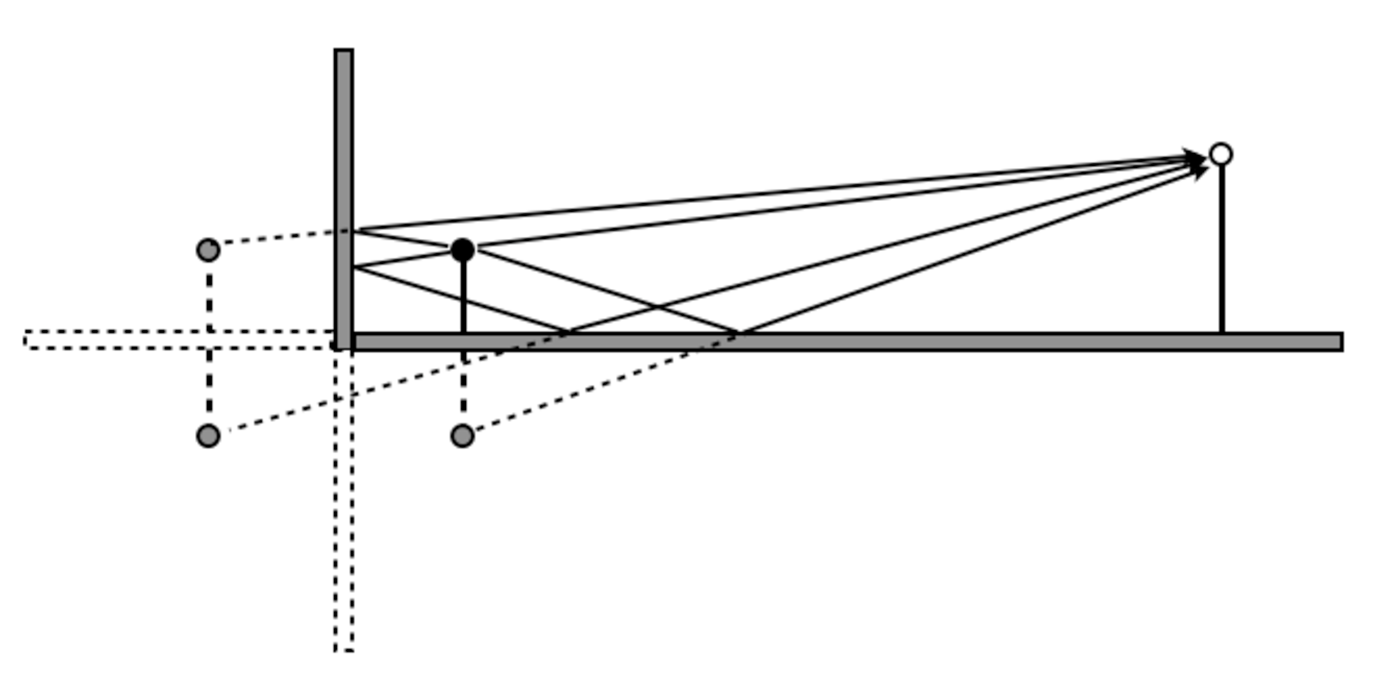
\includegraphics[width=0.9\textwidth]{reflection_floor_wall}
\caption{Direct sound plus reflections off a floor and a back wall.
The reflected sound appears to come from image
sources on the other side of the floor and the other side 
of the back wall.}
\label{f:reflection_floor_wall}
\end{center}
\end{figure}
%
%
\begin{figure}[htbp]
\begin{center}
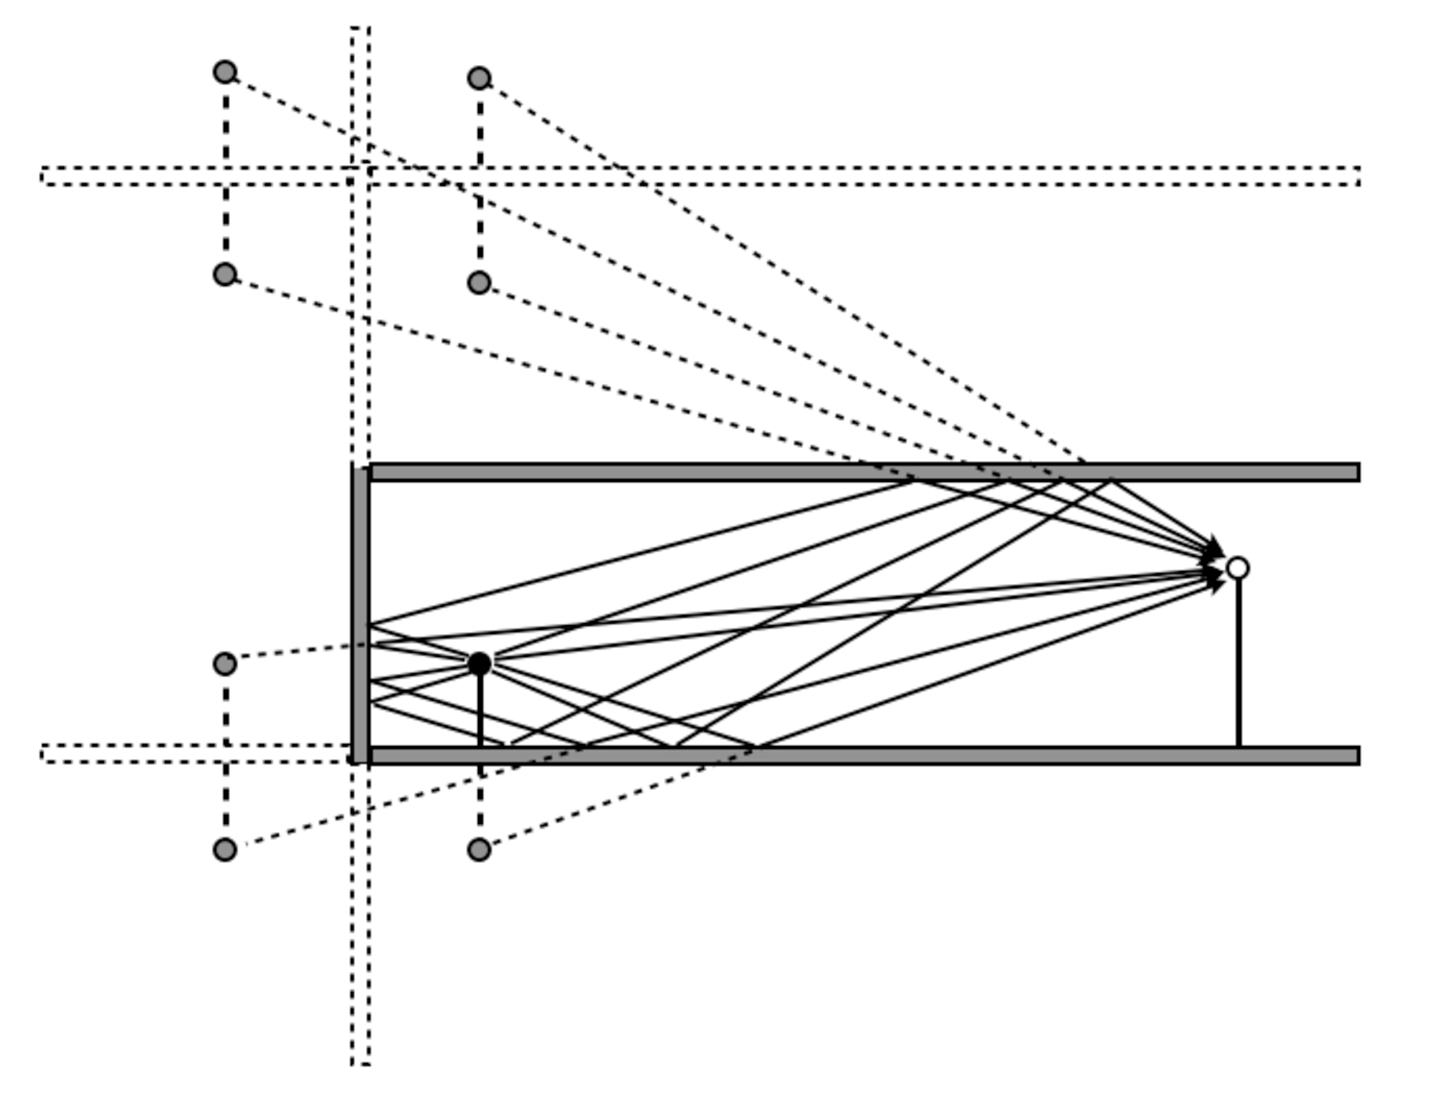
\includegraphics[width=0.9\textwidth]{reflection_floor_wall_ceiling}
\caption{Direct sound plus reflections off a floor, a ceiling,
and a back wall. 
The reflected sound appears to come from image
sources on the other sides of the floor, ceiling, and back wall.}
\label{f:reflection_floor_wall_ceiling}
\end{center}
\end{figure}
%

\ei
%%%%%%%%%%%%%%%%%%%%%%%%%%%%%%%%%%%%%%%%%%%%%%%%%%%%%%
\subsection{Reverberant sound}
\bi

\i {\em Reverberant sound} is the sound that is 
formed from multiple reflections, coming from many 
different directions, and overlapping in time.

\i Figure~\ref{f:reverb_time1} is a graph showing the
direct sound, early reflected sound, and reverberant
sound as a function of time.
Recall that sounds separated by less than 35~msec are
perceived as the same sound.
%
\begin{figure}[htbp]
\begin{center}
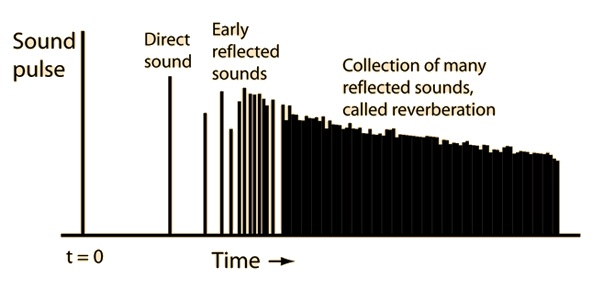
\includegraphics[width=0.8\textwidth]{reverb_time1}
\caption{
A graph showing the distinction between direct,
early reflected, and reverberant sound.
The sound pulse is produced at $t=0$.
The horizontal axis give the arrival time of the
direct and reflected pulse.
The vertical axis is a measure of the sound intensity
level in the direct and reflected sounds.
(Figure taken from  
{http://hyperphysics.phy-astr.gsu.edu/}.)}
\label{f:reverb_time1}
\end{center}
\end{figure}
%

\i The sound intensity level decays as function of time
since the energy in the initial sound pulse is lost by
absorption to the walls, etc.

\i Figure~\ref{f:reverb_time2} shows the build-up and
decay of the sound pressure level ($L_p\approx {\rm SIL}$)
of the reverberant sound for a sustained source of sound.
%
\begin{figure}[htbp]
\begin{center}
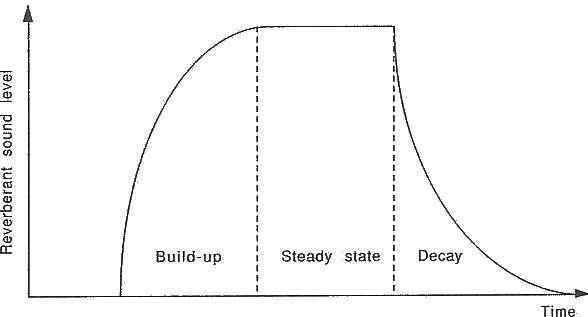
\includegraphics[width=0.8\textwidth]{reverb_time2}
\caption{
Build-up and decay of the sound pressure level 
($L_p\approx{\rm SIL}$) of the
reverberant sound for a sustained source of sound.
D indicates the increase in power due to the arrival
of the direct sound; 1 and 2 are the same for the 
arrival of the first and second reflections.
(Figure taken from  
``Science of Sound," by Rossing, Moore, and Wheeler.)}
\label{f:reverb_time2}
\end{center}
\end{figure}
%

\i The {\em reverberation time} is the time for the 
reverberant sound intensity level to decrease by 60~dB.
This is equivalent to a drop in intensity of the 
reverberant sound by a factor $10^{-6}$ of its 
original value.

\i The reverberation time depends on the frequency 
of the sound.
High frequency sounds typically have 
reverberation times that are less than those for
low frequency sounds.

\i Figure~\ref{f:ideal_reverb} is a graph of ideal
reverberation times for rooms of different sizes and
for various functions.
%
\begin{figure}[htbp]
\begin{center}
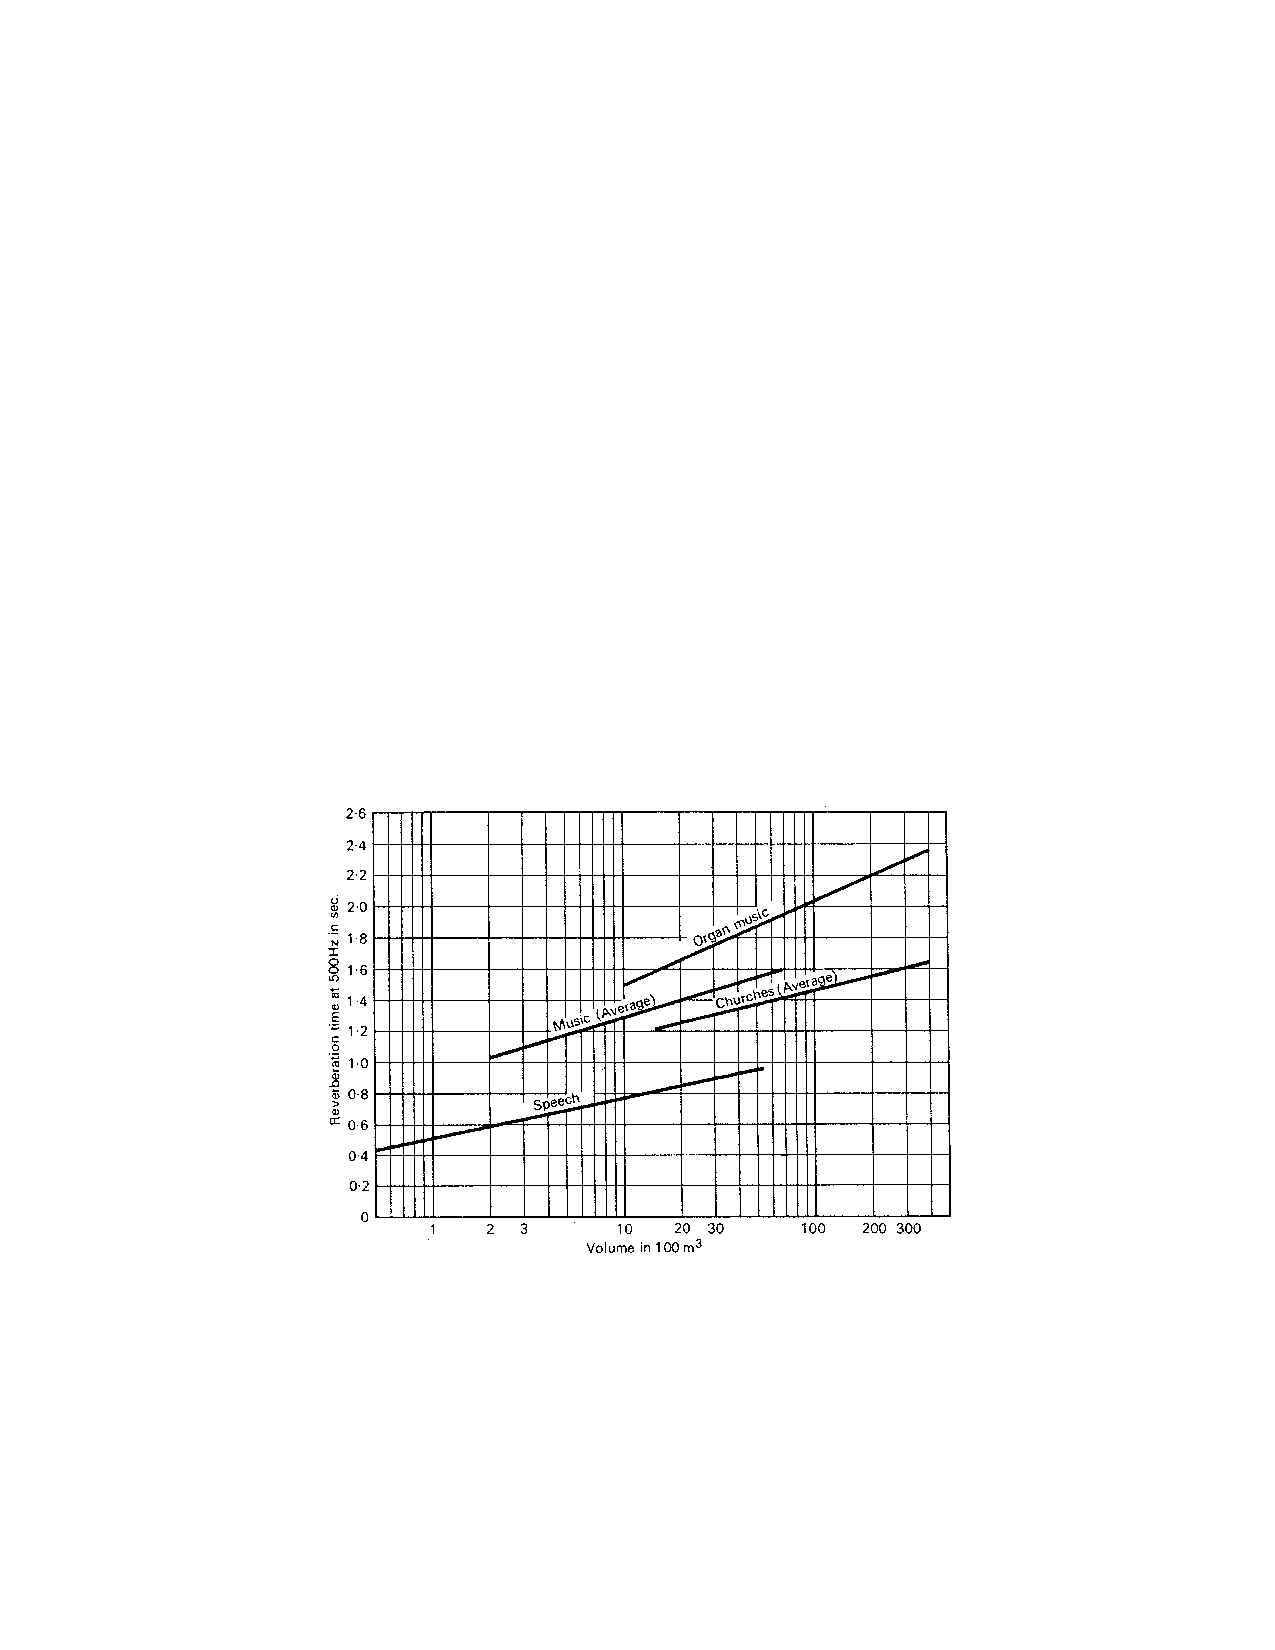
\includegraphics[width=0.8\textwidth]{ideal_reverb}
\caption{Ideal reverberation times for rooms of 
different sizes and for various functions.
(Figure taken from 
``MU1217 Lecture Notes," Cardiff University
by Dr.~Bernard Richardson.)}
\label{f:ideal_reverb}
\end{center}
\end{figure}
%

\i Table~\ref{t:concert_halls} contains 
acoustical characteristics of several different concert halls.
%
\begin{table}[htbp]
\begin{center}
\begin{tabular}{l c c c c c c}
\hline
& Year & Volume & Number & \multicolumn{3}{c}{Reverberation time (sec)}\\
& built & (m${}^3$) & of seats &\multicolumn{3}{c}{\underline{Frequency (Hz)}} \\
&       &           &          & 125 & 500 & 2000 \\
\hline
Teatro alla Scala, Milan  & 1778 & 11,245 & 2289 &     & 1.2 &     \\
Royal Opera House         & 1858 & 12,240 & 2180 &     & 1.1 &     \\
Royal Albert Hall         & 1871 & 86,600 & 6080 & 3.4 & 2.6 & 2.2 \\
Carnegie Hall, New York   & 1891 & 24,250 & 2760 & 1.8 & 1.8 & 1.6 \\
Symphony Hall, Boston     & 1900 & 18,740 & 2630 & 2.2 & 1.8 & 1.7 \\
Royal Festival Hall       & 1951 & 22,000 & 3000 & 1.4 & 1.5 & 1.4 \\
Philharmonic Hall, Berlin & 1963 & 36,030 & 2200 &     & 2.0 &     \\
St.\ David's Hall, Cardiff& 1983 & 22,000 & 2200 & 1.8 & 1.9 & 1.8 \\
\hline
\end{tabular}
\caption{Acoustical characteristics of various
concert halls.
(From a table in
``MU1217 Lecture Notes," Cardiff University
by Dr.~Bernard Richardson.)}
\label{t:concert_halls}
\end{center}
\end{table}
%

\ei
%%%%%%%%%%%%%%%%%%%%%%%%%%%%%%%%%%%%%%%%%%%%%%%%%%%%%%%%%%
\subsection{Calculating the reverberation time}

\bi

\i The reverberation time $T_R$ can be calculated from 
the following formula:
%
\be
T_R = 0.05\,\frac{V}{A_{\rm eff}}~{\rm s}
\ee
%
where $V$ is the total volume of the room (in ft${}^3$)
and $A_{\rm eff}$ is the total absorption (in units of {\em sabin}).

\i Total absorption $A_{\rm eff}$ is given by
%
\be
A_{\rm eff} = A_1 a_1 + A_2 a_2 + \cdots + B_1 + B_2 + \cdots
\ee
%
where $A_i$ and $a_i$ are the surface area (in ft$^2$) 
and absorption coefficient (dimensionless) of surface 
$i=1,2,\dots$
(e.g., the walls, floor, ceiling) in ft$^2$, 
and $B_i$ is the total absorption for chairs, people
in the room, etc.

\i One {\rm sabin} is equivalent to one square-foot of a perfectly 
absorbing surface---e.g., a window one square-foot in area.

\i The sabin is named after Wallace C.\ Sabine (1869-1937), 
who was the
first person to systematically study room acoustics.

\i Note that an absorption coefficient $a=0$
corresponds to no absorption or total reflection.
An absorption coefficient $a=1$ corresponds to 
complete absorption---e.g., an open window or no reflection.

\i The reverberation time depends on the frequency of
the sound, since the absorption coefficients of different
materials depend on frequency.

\i Table~\ref{t:absorption_coefficients} gives the 
absorption coefficients for several different
materials evaluated at different octave intervals.
%
\begin{table}[htbp]
\begin{center}
\begin{tabular}{l c c c c c c}
\hline
& \multicolumn{6}{c}{Frequency (Hz)} \\
Material & 125 & 250 & 500 & 1000 & 2000 & 4000 \\
\hline
Concrete (painted) &
0.10 & 0.05 & 0.06 & 0.07 & 0.09 & 0.08 \\
Plywood panel &
0.28 & 0.22 & 0.17 & 0.09 & 0.10 & 0.11 \\
Plaster on lath &
0.14 & 0.10 & 0.06 & 0.05 & 0.04 & 0.03 \\
Gypsum board, 1/2 in. &
0.29 & 0.10 & 0.05 & 0.04 & 0.07 & 0.09 \\
Glass window &
0.35 & 0.25 & 0.18 & 0.12 & 0.07 & 0.04 \\
Curtains &
0.14 & 0.35 & 0.55 & 0.72 & 0.70 & 0.65 \\
Carpet (on concrete) &
0.02 & 0.06 & 0.14 & 0.37 & 0.60 & 0.65 \\
Carpet (on pad) &
0.08 & 0.24 & 0.57 & 0.69 & 0.71 & 0.73 \\
Acoustical tile, suspended &
0.76 & 0.93 & 0.83 & 0.99 & 0.99 & 0.94 \\
\hline
\end{tabular}
\caption{Absorption coefficients (dimensionless) 
for different materials evaluated at different octave
intervals.
(Based on a similar table in
``Science of Sound," by Rossing, Moore, and Wheeler.)}
\label{t:absorption_coefficients}
\end{center}
\end{table}
%

\i Table~\ref{t:absorption_audience} gives the
absorption (in units of ${\rm m}^2$) for seats and
people in the audience.
To convert to absorption in units of sabin,
multiply the values in the Table by 10.8.
%
\begin{table}[htbp]
\begin{center}
\begin{tabular}{l c c c c c c}
\hline
& \multicolumn{6}{c}{Frequency (Hz)} \\
Material & 125 & 250 & 500 & 1000 & 2000 & 4000 \\
\hline
Wood or metal seat, unoccupied &
0.014 & 0.018 & 0.020 & 0.036 & 0.035 & 0.028 \\
Upholstered seat, unoccupied &
0.13 & 0.26 & 0.39 & 0.46 & 0.43 & 0.41 \\
Adult &
0.23 & 0.32 & 0.39 & 0.43 & 0.46 & --- \\
Adult in an upholstered seat &
0.27 & 0.40 & 0.56 & 0.65 & 0.64 & 0.56 \\
\hline
\end{tabular}
\caption{Absorption (in units of ${\rm m}^2$) 
for different types of seats with and without people 
evaluated at different octave intervals.
To convert to absorption in units of sabin, 
multiply the values in the Table by 10.8.
(Based on a similar table in
``Science of Sound," by Rossing, Moore, and Wheeler.)}
\label{t:absorption_audience}
\end{center}
\end{table}

\i \exer
Calculate the reverberation time at $500~{\rm Hz}$ for a room
with dimensions $20~{\rm m}\times 15~{\rm m}\times 8{\rm m}$ (high).
The walls are painted concrete, the ceiling is plaster,
and the floor is carpet on pad.
Also, assume that there are 200~upholstered seats, and that
they are half-filled with people.

\i \ans
First converting to units of feet, and 
using data from Tables~\ref{t:absorption_coefficients} and 
\ref{t:absorption_audience} at $f=500~{\rm Hz}$:
%
\begin{align}
L&= 20~{\rm m}\times 3.28~{\rm ft/m} = 65.6~{\rm ft}
\\
W&=15~{\rm m}\times 3.28~{\rm ft/m} = 49.2~{\rm ft}
\\
H&=8~{\rm m}\times 3.28~{\rm ft/m} = 26.24~{\rm ft}
\\
V&=L\times W\times H =2400~{\rm m}^3
=8.47\times 10^4~{\rm ft}^3
\\
A_{\rm eff}&= 
0.06\left[2(L\times H) + 2(W\times H)\right]
+0.06 (L\times W) + 0.57 (L\times W)
\nonumber\\
&\quad + 10.8(100\times 0.39 + 100\times 0.56)
\nonumber\\
&= 3.42\times 10^3~{\rm sabin}
\\
T_R &= 1.2~{\rm sec}
\end{align}

\i Comparing with Figure~\ref{f:ideal_reverb}, we see that this
value for $T_R$ is close to ideal for music (average) for a room 
of this volume ($2400~{\rm m}^3$).

\ei

%%%%%%%%%%%%%%%%%%%%%%%%%%%%%%%%%%%%%%%%%%%%%%%%%%
\subsection{Criteria for good acoustical design}
\bi

\i \underline{Adequate loudness}: 
Everybody in the audience should be able to hear the 
speaker or the performers.
The room shouldn't be too large or be too absorptive.

\i \underline{Uniformity}: 
The sound should be spread uniformly throughout the 
room.
There shouldn't be ``live" spots or ``dead" spots
in the room.

\i \underline{Reverberance or liveness}:
The reverberation time should be sufficiently large 
so that the listener feels bathed in sound from all 
directions.

\i \underline{Clarity}:
The reverberation time shouldn't be so large that 
the revererberant sound masks subsequent sounds.
(Clarity and reverberance are competing qualities.)

\i \underline{Freedom from echoes}:
The room should be free of echoes.

\i \underline{Freedom from background noise}:
The room should be free of excessive levels of 
background or external noise.

\ei
%%%%%%%%%%%%%%%%%%%%%%%%%%%%%%%%%%%
\subsection{Problems to avoid}
\bi

\i \underline{Echoes}: 
Reflected sounds should arrive early 
enough ($<35~{\rm msec}$) in order to avoid echoes.

\i Since curved surfaces tend to focus sound to 
certain areas in a room, these should be avoided.

\i Figure~\ref{f:whispering_chamber} shows how 
sound produced at one focal point of a room 
with elliptical walls is focused at the 
other focal point. 
%
\begin{figure}[htbp]
\begin{center}
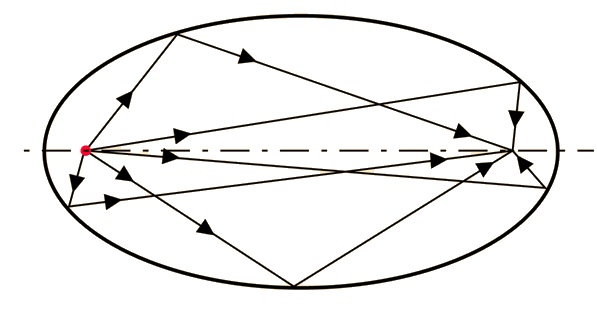
\includegraphics[width=0.8\textwidth]{whispering_chamber}
\caption{Illustration of the so-called
``whispering chamber effect"
for a room shaped like an ellipse (top view).
The whisperer sits at the focal point indicated by
the red dot, and listener sit at the other focal point.
(Figure taken from  
{http://hyperphysics.phy-astr.gsu.edu/}.)}
\label{f:whispering_chamber}
\end{center}
\end{figure}
%

\i Parallel walls can produce {\em flutter echoes}
since there are multiple paths for the reflected sound
to reach the listener, corresponding to an 
infinite number of image sources.
See Figure~\ref{f:reflections_parallel}. 
%
\begin{figure}[htbp]
\begin{center}
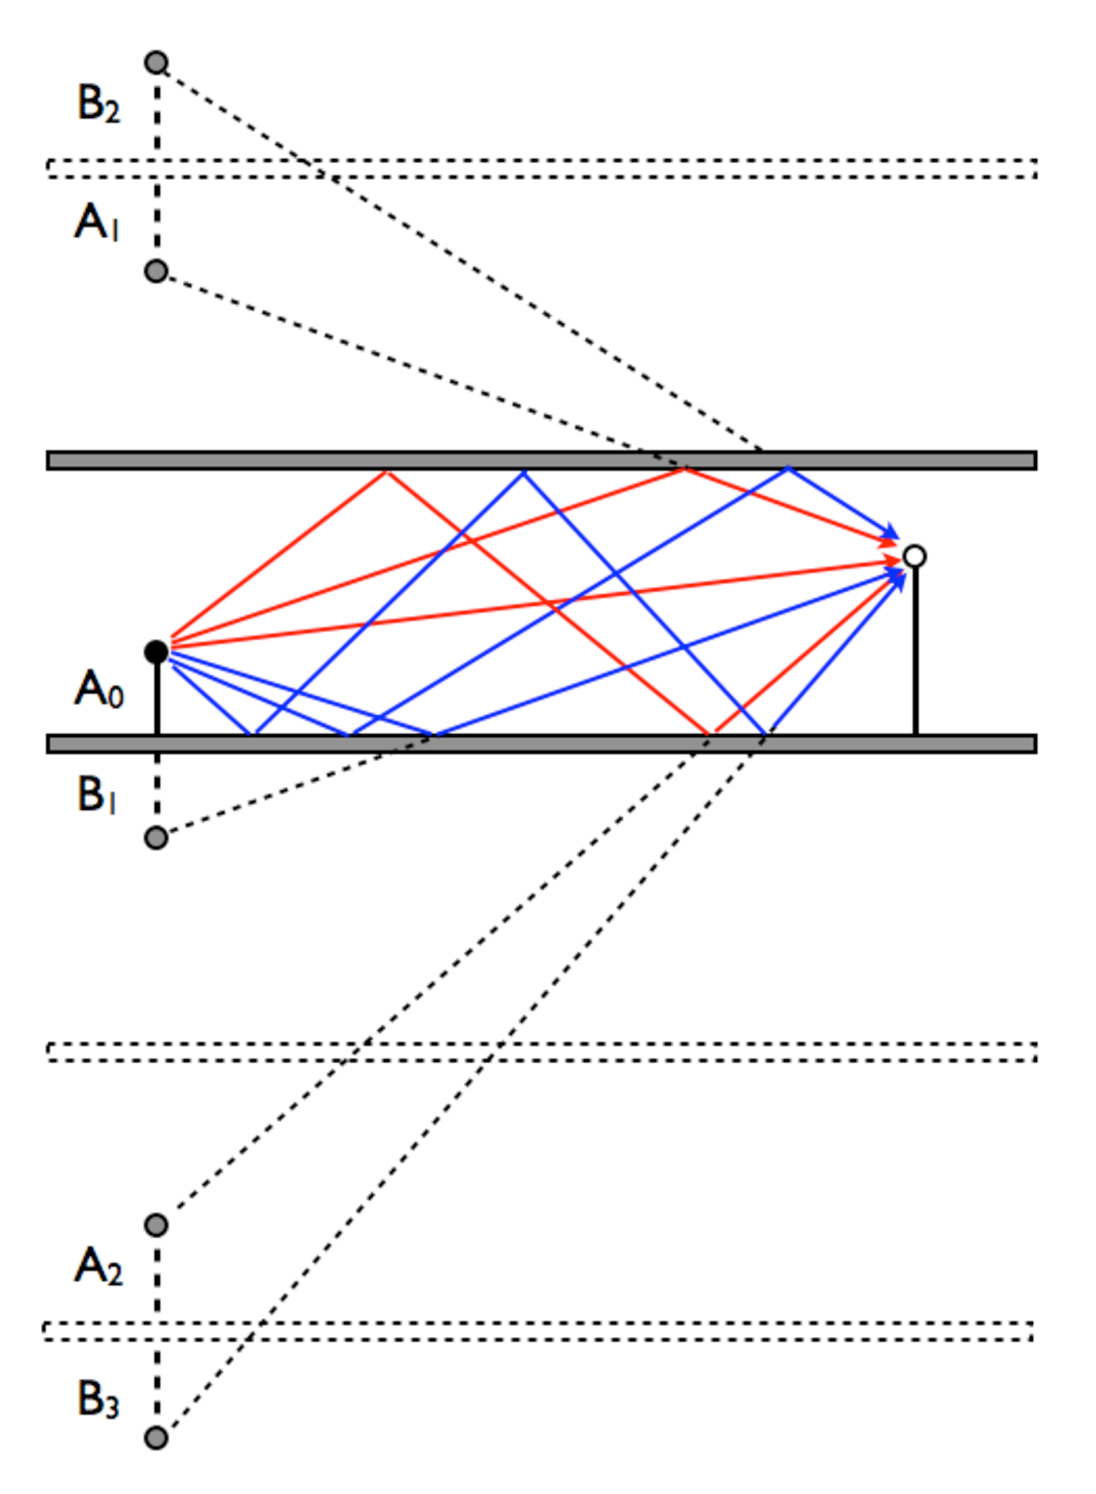
\includegraphics[width=0.9\textwidth]{reflections_parallel}
\caption{Multiple reflections and image sources due to 
parallel floor and ceiling.
Multiple reflections from closely-spaced parallel surfaces
can produce so-called flutter echoes.}
\label{f:reflections_parallel}
\end{center}
\end{figure}
%

\i \underline{Shadows}:
Sound shadows produced by overhanging balconies or columns
in the room should be avoided as much as possible.

\i \underline{Resonances}:
Room resonances should be avoided as much as possible,
since they would distort (i.e., filter) the sound 
produced by the source.
One can avoid room resonances by {\em not} having parallel walls 
and ceilings.

\i Note that a rectangular box-shaped room with 
dimensions $L\times W\times H$
would have resonances at the discrete frequencies
%
\be
f_{lmn} = \frac{v}{2}
\sqrt{\left(\frac{l}{L}\right)^2 
+\left(\frac{m}{W}\right)^2 
+\left(\frac{n}{H}\right)^2}\,,
\qquad
l, m, n =1,2,3\cdots
\ee
%
where $v$ is the speed of sound in air.
(This is just a generalization of standing waves in 
a 1-dimensional tube closed a both ends to 3 dimensions.)

\i \exer
Calculate the first few resonant frequencies for a 
rectangular-shaped shower stall having dimensions 
$1~{\rm m}\times 1~{\rm m}\times 2{\rm m}$.

\i \ans
%
\begin{align}
&f_{001}=85~{\rm Hz}\,,\quad
f_{010}=170~{\rm Hz}\,,\quad
f_{100}=170~{\rm Hz}\,,\quad
\\
&f_{002}=170~{\rm Hz}\,,\quad
f_{110}=240~{\rm Hz}\,,\quad
f_{111}=255~{\rm Hz}\,,\cdots
\end{align}

\i Although resonances might be good for singing in the 
shower, they are not good for concert halls in general!

\i \underline{Background noise}:
External noise due to heating, ventillation or air conditioning
systems should be kept to a minimum.

\i For example, one should try to isolate the air conditioning 
unit from the ceiling joists, which would strongly couple the 
vibrations of the air conditioning unit into the building.
 
\ei
%%%%%%%%%%%%%%%%%%%%%%%%%%%%%%%%%%%%%%%%%%%%%%%%%%%%%%%%%%%
\subsection{Terminology used for concert halls}
\bi

\i \underline{Intimacy or presence}:
The impression of being in a small concert hall.

\i \underline{Spaciousness}:
The sound appears to come from all directions and
from a source wider than the visual width of the source.

\i \underline{Reverberance or liveness}:
(As before.)
The feeling that the listener is bathed in sound.

\i \underline{Clarity}:
(As before.)
Being able to distinguish between discrete sounds in a musical
performance.

\i \underline{Warmth}:
Liveness of the bass notes (75~Hz--350~Hz) relative to the
treble notes.

\i \underline{Brilliance}:
Liveness of the treble notes ($>350~{\rm Hz}$) relative to the
bass notes.

\i \underline{Blend}:
Mixing of sounds from different instruments.

\i \underline{Ensemble}:
The ability of the performers to hear and respond to music
that they hear from the other performers.
A time delay of $< 50~{\rm msec}$ between notes 
requires the performing stage to be $< 50~{\rm ft}$.

\ei

